\cleardoublepage
\singlespacing
\chapter{EVALUATION \& RESULTS}
\label{c:evaluation}
\doublespacing\nointerlineskip

%This chapter presents evaluation. The models and algorithms are
%tested extensively on benchmarks, which is described in
%section~\ref{s:benchmarks}, and the results are discussed in
%section~\ref{s:results}


The performance of the fault tolerance system is evaluated with the metrics listed below:
\begin{enumerate}
\item Correctness, whether the system is configured to do what the mapping result specifies, including the heartbeats, heartbeat periods, recovery chains, application links.
\item Communication overhead used for heartbeats
\item Communication overhead for failure recovery
\item Failure detection success rate
\item Fault recovery success rate
\item The average time to recover from the time of failure
\item The average number of messages used to recover the system
\end{enumerate}

In order to evaluate the performance of the fault tolerant system on RASCO and Strips, application shown in Figure~\ref{fid:application} will be deployed through WuKong. First we describe the hardware platform that will be hosting the Strips, then we describe the experimental setup for the deployment. Lastly, we present the results with discussion.

\subsection{Hardware Platform}

\begin{figure}[h!]
\caption{An WuDevice}
\label{fig:wudevice}
\centering
    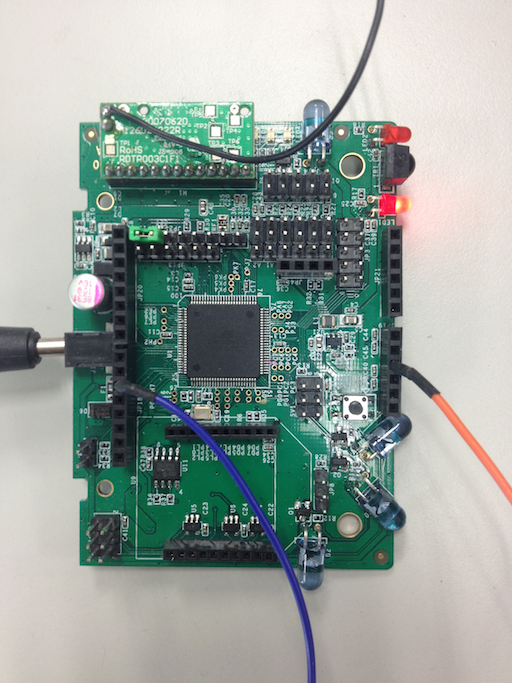
\includegraphics[width=\linewidth]{figures/wudevice}
\end{figure}

All boards are equipped with an Atmel ATmega1280-16AU 8-bit microcontroller with 4K of EEPROM and 64k of flash. The boards hardware design is based upon Arduino hardware referenced design, in addition, every board has wires for mounting multiple wireless protocol adapters such as ZWave, ZigBee. In the following experiments, every board is only equipped with a ZWave adapter, and only communicating through ZWave. 

Every board is also pre-installed with a modified version of NanoVM (ref here) called “NanoKong” that supports all the basic WuKong framework protocols including the new additions from the work in the previous chapter.

A PC with wireless access is dedicated for hosting the WuKong Master software which is responsible for managing WuKong applications for the whole system and serves as a mean to present an interface to the users.

Three boards will be used in the experiments below. One of them is equipped with a light sensor that returns a byte indicating the light level around the sensor. The rest are equipped with a relay which each controls the power supply of a lamp.

An additional board with the same hardware specification is used as a gateway between the Master and the sensor network.

\subsection{Experimental Setup}

% we could do it today
Three WuDevices are deployed in a room where two of them are connected to a 

%Describe limits: 
%1. Fully connected network

In this experiment, an application shown in figure 1 above will be deployed with a fault tolerance user policy shown in the figure 2 upon the hardware setup described in the previous section three times to evaluate its performance.

The application requires a light sensor and a light actuator. The light actuator will turn on the light if the sensed light value is below a threshold specified from the numeric controller. Numeric controller is fixed on a value of 200. The light value takes a byte ranging from 0 to 255. The comparison is done with a virtual component Threshold in native implementation.

We will simulate a node failure by unplugging the power supply of the active light sensor node on all tries.

\section{Results}
\label{s:results}

Blah blah, show and discuss results and data here
